% !TEX encoding = UTF-8 Unicode
% !BIB TS-program = biber
%
% This file is MIT-Thesis.tex, a LaTeX template for formatting an MIT thesis with the mitthesis class.
%
% Version: 1.23, 2026/05/05
%
% Author: John H. Lienhard, copyright 2026. Reuse under the MIT license: https://ctan.org/license/mit 
%
% DOCUMENTATION is here: https://ctan.org/pkg/mitthesis
%
% This package requires TeX Live 2022 or later.


%% Don't remove the \DocumentMetadata command 
\DocumentMetadata
{
	lang		= en-US, % default language
	pdfversion  = 1.7,
	pdfstandard = a-2b,
%	pdfversion  = 2.0,   % default version
%	pdfstandard = { ua-2, a-4f }, % requires pdfversion  = 2.0; requires TeX Live 2024 or later.
%	tagging		= on, % For tagging (accessible PDF), run lualatex with TeX Live 2025 or later.
					  % Do not include appendixa.tex when selecting this option (listings package is not compatible).
%	debug		= { xmp-export }, % if you want to check your metadata (xmpi file).
}

%%%%%%%%%  Documentclass and options  %%%%%%%%%%%%%%%%%%%%%%%%%%%%%%%%%%%%%

\documentclass[twoside]{mitthesis}
% 						fontset=libertinus, fontset=lmodern, fontset=lucida, 
%						fontset=fira-newtxsf, fontset=newtx, fontset=newtx-sans-text,  
%						fontset=heros-stix2,  fontset=stix2, fontset=termes-stix2, fontset=termes
%
% option [twoside]		gives facing-page behavior for printing; omitting twoside will eliminate even-numbered blank pages
%						(use mydesign to change page margins, e.g., for binding).
%
% option [lineno]	 	provides line numbers, as for editing
%
% option [fontset=xxx]  is a keyvalue which can be:
%					 	for pdftex or lualatex engine:  defaultfonts, libertinus, lmodern, lucida
%					 	for pdftex only: 				fira-newtxsf, newtx, newtx-sans-text
%						for lualatex only:				heros-stix2, stix2, termes, termes-stix2
%					 	if no key value is given, fonts default to CMR (pdftex) or LMR (unicode), i.e., "the LaTeX font".
%					 	You can edit the fontset files or you can write your own, myfonts.tex, and do [fontset=myfonts].
%						If you are using multiple languages, load the babel package in your fontset file, before the fonts.
%
% option [mydesign] 	loads packages for color, title and list formats, margins, or captions. 
%	or [mydesign=file]	You can edit mydesign.tex to change defaults. Other design files can be loaded as
%						key values, [mydesign=filename], where filename.tex should be in your working directory.
%						Two example files are provided: mydesign_redsans_headings.tex and mydesign_libertinus_headings.
%						See documentation for details and a description of the appropriate fontsets to use with each.
%
%					    As distributed, mydesign.tex will set caption labels in bold face (e.g., "Figure 1.1:" in bold)
%

%%%%%%%%  Packages used in the sample chapters (not otherwise required) %%%

%% Package for code listing in Appendix A.
\usepackage{listings}%   documentation is here https://ctan.org/pkg/listings

%% Set chemical formulas nicely
\usepackage[version=4]{mhchem}%   documentation at https://ctan.org/pkg/mhchem

%% Pseudocode for the learning algorithms (Chapter 4)
\usepackage{algorithm}%       float environment (https://ctan.org/pkg/algorithms)
\usepackage{algpseudocodex}%  pseudocode body (https://ctan.org/pkg/algpseudocodex)
  \floatname{algorithm}{Algorithm}
  \algrenewcommand\algorithmicrequire{\textbf{Input:}}
  \algrenewcommand\algorithmicensure{\textbf{Output:}}

%% Latin filler used in Chapter 1, with a test for package version date (https://ctan.org/pkg/lipsum)
\usepackage{lipsum}
\IfPackageAtLeastTF{lipsum}{2021/09/20}{\setlipsum{auto-lang=false}}{} % to avoid a hyphenation warning


%%%%%%%%%  Other optional packages used sample chapters  %%%%%%%%%%%%%%%%%%

%% Table related packages  

\usepackage{booktabs}% publication quality tables (https://ctan.org/pkg/booktabs)

\usepackage{array}% Additional options for column formats (https://ctan.org/pkg/array)

\usepackage{dcolumn}% For alignment of numbers on the decimal place (https://ctan.org/pkg/dcolumn) 
  \newcolumntype{d}[1]{D{.}{.}{#1}}% use with dcolumn package. Note: dcolumns are set in math mode.
  % syntax: d{x.y} where x is max number of digits before decimal and y is max number after.

% Package for multipage table in Appendix B.
\usepackage{longtable}% typeset multi-page tables (https://ctan.org/pkg/longtable)
	\setlength{\LTcapwidth}{\linewidth}% width of caption over longtables.  Adjust as desired.

%\usepackage{tabularx}% adjustable-width columns in tabular (https://ctan.org/pkg/tabularx)

%% Package for improved typography
\usepackage[nopatch=footnote]{microtype}% typographic fine-tuning (https://ctan.org/pkg/microtype)
										% https://github.com/latex3/tagging-project/issues/67#issue-2163508995

%% Load this package if using the two-column nomenclature format, \begin{nomenclature*}
\usepackage{multicol}

\usepackage{tikz}% vector diagrams drawn inline (https://ctan.org/pkg/pgf)
\usetikzlibrary{arrows.meta}


%%%%%%%%%  Graphics path (to figure files)  %%%%%%%%%%%%%%%%%%%%%%%%%%%%%%%%

%% Can set graphicspath to point to specific directories containing figures (the current directory is searched automatically)
%% For instance, to search a subdirectory of the current directory called "figures" and a parallel directory called "art", set:

% \graphicspath{ {figures/} {../art/} }% For details see: https://latexref.xyz/dev/latex2e.html#g_t_005cgraphicspath


%%%%%%%%%  Representative set-up for biblatex  %%%%%%%%%%%%%%%%%%%%%%%%%%%%%

%% biblatex is very powerful, and you can customize most aspects the reference list and citations to suit your needs.
%%   documentation is here: https://ctan.org/pkg/biblatex
%%   cheat sheet is here:   https://tug.ctan.org/info/biblatex-cheatsheet/biblatex-cheatsheet.pdf

%% Numerical citations of references
\usepackage[style=ext-numeric-comp,giveninits=true,maxbibnames=10,sorting=none,language=american]{biblatex}

% and make some changes to that style
	\renewcommand{\multicitedelim}{\addcomma}% removes space between consecutive cites to give [6,7], not [6, 7]
    \AtEveryBibitem{%
      \ifentrytype{article}{%
        \renewbibmacro{in:}{}% Removes "In:" for articles
		\renewcommand*{\jourvoldelim}{\addcomma\space}   % put comma after journal title
		\renewcommand*{\volnumdatedelim}{\addcomma\space}% put comma after volume info
		\renewbibmacro*{issue+date}{% Print date without parentheses around it
		\iffieldundef{issue}%
        	{}%
        	{\printfield{issue}%
         	\setunit*{\addcomma\space}
        	}%
			\printdate
		}
      }{}
    }
    %
	\renewbibmacro*{volume+number+eid}{%
        \printtext[bold]{\printfield{volume}}%    bold volume (issue number) , eid
%        \printtext[parens]{\printfield{number}}%  
        \iffieldundef{number}
          {} % do nothing
          {\printtext[parens]{\printfield{number}}} % print number in parentheses
        \setunit{\bibeidpunct}%
        \printfield{eid}
    }

%% IEEE style citations and references
% \usepackage[style=ieee,maxbibnames=10,sorting=none]{biblatex}% style=ext-numeric-comp,articlein=false,giveninits=true
%	 \DefineBibliographyStrings{english}{url= \textsc{url} ,  }% replaces the IEEE default "[Online]. Available" by "URL"

%% author-year style citations and references 
%% use \parencite, not \cite, when you want "(Author, year)"
%% The sample files are not set up to include parentheses.
% \usepackage[style=authoryear, maxbibnames=10]{biblatex} 


\addbibresource{references.bib}%% <== change to YOUR bib file <========= CHANGE !!


%% to avoid split urls and stretched white space, you can make the bibliography ragged-right by uncommenting this:
%\AddToHook{cmd/bibsetup/after}{\raggedright}

%% To ensure citations are set, run Latex --> biblatex --> Latex again (unless your installation does this automatically)


%%%%%%%%%%  Option for "double spacing" %%%%%%%%%%%%%%%%%%%%%%%%%%%%%%%%%%%%

%% Back in the typewriter era, double spaced lines were convenient for editing with a pencil. 
%% In typography, the separation between lines is called "leading", and it is usually set in 
%% proportion to the font size (i.e., when the font is loaded).  If you really feel the need 
%% to change the line separation, the most attractive results will be obtained by changing the
%% leading in proportion to the the current font size, rather than just doubling the space.

%% The setspace package provides a tool for changing line separation. Use these two commands here:
%
% \usepackage{setspace}%  documentation at https://ctan.org/pkg/setspace
% \setstretch{1.1}% you can choose some other value for the stretch of space between lines
%
%% Use one or more of the these commands *AFTER* the frontmatter
%
% \onehalfspacing
% \doublespacing
% \singlespacing  % will turn these effects off (you can use these anywhere in the document)

%% The best result is usually to stay with the default leading (or to learn about latex font settings).


%%%%%%%%%%%  Metadata  %%%%%%%%%%%%%%%%%%%%%%%%%%%%%%%%%%%%%%%%%%%%%%%%%%%%%%%

% Most of the document metadata is created automatically. 
% The following items should be adjusted to match your work. <================= !!!!!!!!!!

\hypersetup{%
	pdfsubject={MSs Thesis in Data Science and Artificial Intelligence, Christian Faccio},
	% Change this to briefly state topic of your thesis 
% 
	pdfkeywords={University of Trieste, MSc Thesis, Data Science, Artificial Intelligence, Underwater Search and Navigation},
	% Add keywords that will help search engines and libraries to find your work.
	% Includes the name[s] of the author[s] 
	% (If you used \DocumentMetadata at line 14, you can just put "\CopyrightAuthor," for the names.)
%
	pdfurl={https://github.com/christianfaccio/MSc_Thesis.git},
	% If you have a url for the thesis, put it here. Otherwise delete this.
	% (MIT Libraries will put your thesis in DSPACE with a persistent url after you submit it.)
%	
	pdfcontactemail={christianfaccio@outlook.it},
	% You can put a [permanent] email address into the metadata, if you like.
	% Otherwise delete this.
%
	pdfauthortitle={},
	% If you have a title (e.g., Prof. Dr.-Ing.), you can include it here.
}

%%%%%%%%%%%%  Math operators %%%%%%%%%%%%%%%%%%%%%%%%%%%%%%%%%%%%%%%%%%%%%%%%%%%%

% These commands declare two math operators, \erf{..} and \erfc{..} using the mathtools package.
% note: * form, \erf*{..}, produces automatic delimiter scaling; 
%       optional argument sets size manually, e.g. \erf[\bigg]{..}.
% See Table 1.1 in Chapter 1

\DeclareMathOperator{\Erf}{erf}
\DeclareMathOperator{\Erfc}{erfc}
\DeclarePairedDelimiterXPP\erf[1]{\Erf\mkern1mu}(){}{#1}% increase to 2mu with stix2 font
\DeclarePairedDelimiterXPP\erfc[1]{\Erfc\mkern1mu}(){}{#1}


%%%%%%%%%%%%  UniTS title page  %%%%%%%%%%%%%%%%%%%%%%%%%%%%%%%%%%%%%%%%%%%%%%%%%

% Replaces the MIT title page with the layout of the official UniTS
% "frontespizio_tesi" template. Everything else in mitthesis is unchanged.
% The UniTS fields are set below, next to \title.

% frontespizio.tex
%
% UniTS (Università degli Studi di Trieste) title page for the mitthesis class.
% Reproduces the layout of the official "frontespizio_tesi.doc" template:
%
%       [ logos ]
%       Dipartimento di ...            (Arial bold 16pt, centered)
%       CORSO DI LAUREA ...            (Arial bold 16pt, centered)
%       TESI DI LAUREA MAGISTRALE      (Arial bold 16pt, centered)
%       TITLE                          (Arial bold 20pt, centered)
%       Graduating student:   Supervisor:    (Arial italic 16pt, names bold;
%       Name                  Name            the pair is centered on the page)
%                             Co-supervisor:
%                             Name
%       ANNO ACCADEMICO 20.. - 20..    (Arial bold italic 12pt, centered)
%
% This file only replaces \maketitle. Everything else in mitthesis (abstract page,
% headings, TOC, bibliography, ...) is untouched, so the MIT abstract page still
% uses \Author, \Degree and \Supervisor -- keep those commands in main.tex.
%
% \input this file in the PREAMBLE of main.tex, then set the fields below after
% \begin{document} and before \maketitle.

\ProvidesFile{frontespizio.tex}[2026/07/27 v1.0 UniTS title page for mitthesis]

%%%%%%%%%%  Arial-like sans serif  %%%%%%%%%%%%%%%%%%%%%%%%%%%%%%%%%%%%%%%%%%%
%
% The Word template uses Arial, which is not free. We substitute a metrically
% compatible Helvetica clone. Both branches only change \sffamily, not the body
% text font, and both embed fully (so PDF/A-2b conformance is preserved).
%
%   pdflatex  -> helvet (URW Nimbus Sans, Type 1)
%   lualatex  -> TeX Gyre Heros (OpenType) via fontspec; helvet cannot be used
%                with a Unicode engine (there is no TU/phv font definition, and
%                \sffamily would silently fall back to Latin Modern *serif*).

\usepackage{iftex}
\ifPDFTeX
	\usepackage[scaled]{helvet}
\else
	\usepackage{fontspec}
	\setsansfont{texgyreheros}[
		Extension      = .otf,
		UprightFont    = *-regular,
		BoldFont       = *-bold,
		ItalicFont     = *-italic,
		BoldItalicFont = *-bolditalic,
		Scale          = MatchLowercase,
	]
\fi

%%%%%%%%%%  UniTS title page fields  %%%%%%%%%%%%%%%%%%%%%%%%%%%%%%%%%%%%%%%%%

\newcommand*\UNITSdipartimento{}
\newcommand*\Dipartimento[1]{\renewcommand*\UNITSdipartimento{#1}}

\newcommand*\UNITScorso{}
\newcommand*\CorsoDiLaurea[1]{\renewcommand*\UNITScorso{#1}}

% "PROVA FINALE" for a bachelor's, "TESI DI LAUREA MAGISTRALE" for a master's
\newcommand*\UNITStipotesi{TESI DI LAUREA MAGISTRALE}
\newcommand*\TipoTesi[1]{\renewcommand*\UNITStipotesi{#1}}

% \Laureando[Laureanda]{Name} -- optional argument overrides the label
\newcommand*\UNITSlaureando{\CopyrightAuthor}
\newcommand*\UNITSlaureandolabel{Laureando}
\newcommand*\Laureando[2][Graduating student]{%
	\renewcommand*\UNITSlaureandolabel{#1}%
	\renewcommand*\UNITSlaureando{#2}%
}

% Separate multiple names with \\ if needed
\newcommand*\UNITSrelatore{}
\newcommand*\Relatore[1]{\renewcommand*\UNITSrelatore{#1}}

\newcommand*\UNITScorrelatore{}
\newcommand*\Correlatore[1]{\renewcommand*\UNITScorrelatore{#1}}

% \AnnoAccademico{2025}{2026}
\newcommand*\UNITSanno{}
\newcommand*\AnnoAccademico[2]{\renewcommand*\UNITSanno{#1 -- #2}}

%%%%%%%%%%  Logos  %%%%%%%%%%%%%%%%%%%%%%%%%%%%%%%%%%%%%%%%%%%%%%%%%%%%%%%%%%%
%
% Default: UniTS on the left, partner institution on the right, both at the same
% optical height. Redefine \UNITSlogos in main.tex for a different arrangement
% (e.g. a single centered logo, or a third logo).

\newcommand*\UNITSlogoheight{16mm}

% Horizontal gap between the two columns of the "student / supervisor" block.
% The columns themselves shrink to fit their text, and the resulting pair is
% centered on the page, so this is the only knob: increase it to spread the
% columns apart, decrease it to pull them together.
\newcommand*\UNITSsignaturegap{60mm}

\newcommand\UNITSlogos{%
	\noindent
	\begin{minipage}{\textwidth}%
		\centering
		
\includegraphics[height=\UNITSlogoheight]{assets/logoTS.png}%
		\hfill
		
\includegraphics[height=\UNITSlogoheight]{assets/logoUA.png}%
	\end{minipage}%
	\par
}

%%%%%%%%%%  Access to the title  %%%%%%%%%%%%%%%%%%%%%%%%%%%%%%%%%%%%%%%%%%%%%
%
% We read the class' own title variable rather than \@title: older mitthesis
% releases (e.g. the one shipped with TeX Live 2024) never set \@title, so using
% it raises "LaTeX Error: No \title given".

\ExplSyntaxOn
\cs_new:Npn \UNITStitle { \tl_use:N \g_mitthesis_title_tl }
\ExplSyntaxOff

%%%%%%%%%%  The title page itself  %%%%%%%%%%%%%%%%%%%%%%%%%%%%%%%%%%%%%%%%%%%
%
% The starred form \maketitle* is accepted for compatibility with mitthesis
% (where it suppressed the MIT copyright-permission paragraph); here there is
% no copyright block, so the star has no effect.

\makeatletter
\RenewDocumentCommand\maketitle{s}{%
	\clearpage
	\thispagestyle{empty}
	\pdfbookmark[0]{Frontespizio}{titlepage}
	%
	\begingroup
	\sffamily
	\setlength{\parindent}{0pt}%
	\centering
	%
	\UNITSlogos
	%
	\vspace{14mm}
	%
	{\fontsize{16}{19}\selectfont\bfseries \UNITSdipartimento \par}
	\vspace{7mm}
	{\fontsize{16}{19}\selectfont\bfseries \UNITScorso \par}
	\vspace{7mm}
	{\fontsize{16}{19}\selectfont\bfseries \UNITStipotesi \par}
	%
	\vspace{24mm}
	%
	{\fontsize{20}{24}\selectfont\bfseries \UNITStitle \par}
	%
	\vspace{28mm}
	%
	% Graduating student on the left, supervisor/co-supervisor on the right.
	% Each column is a tabular, so it is exactly as wide as its own longest line
	% (fixed-width minipages would pad the right column with empty space and
	% push the visible block off-center). The pair is then centered as a unit by
	% the \centering in force. Labels are italic, names are bold italic.
	{\fontsize{16}{19}\selectfont\itshape
		\begin{tabular}[t]{@{}l@{}}
			\UNITSlaureandolabel: \\[0.4ex]
			\textbf{\UNITSlaureando}
		\end{tabular}%
		\hspace{\UNITSsignaturegap}%
		\begin{tabular}[t]{@{}l@{}}
			Supervisor: \\[0.4ex]
			\textbf{\UNITSrelatore}
			\ifx\UNITScorrelatore\@empty\else
				\\[1.4ex] Co-supervisor: \\[0.4ex]
				\textbf{\UNITScorrelatore}
			\fi
		\end{tabular}%
		\par
	}
	%
	\vfill
	%
	{\fontsize{12}{14}\selectfont\bfseries\itshape
		ACADEMIC YEAR \UNITSanno \par}
	%
	\vspace{4mm}
	\endgroup
	%
	% Metadata that mitthesis normally sets inside its own \maketitle.
	\hypersetup{%
		pdfauthor={\CopyrightAuthor},
		pdfcaptionwriter={\CopyrightAuthor},
	}%
	\cleardoublepage
	% NB: mitthesis' automatic "Thesis Committee" page is deliberately NOT
	% generated here -- it is MIT-specific. \Reader entries are ignored.
}
\makeatother



%%%%%%%%%%%%  Abstract page adjustments  %%%%%%%%%%%%%%%%%%%%%%%%%%%%%%%%%%%%%%%%

% Two changes to the mitthesis abstract page:
%   1. drop the submission date from the "Submitted to the Department ..." line;
%   2. drop the "Thesis supervisor / Title" block printed after the abstract text.
% \ThesisDate and \Supervisor must still be given below: the class requires them,
% and they are used by other (unprinted) mitthesis pages.

\ExplSyntaxOn

% Same as the class definition, minus "on <thesis date>".
\cs_set_protected:Nn \__mitthesis_degree_abstractblock: {
	\int_set:Nn  \l_tmpa_int {1}
	\int_set:Nn  \l_tmpb_int {1}
	\tl_set:Ne \l_tmpa_tl { \seq_item:NV \g__mitthesis_degree_dept_seq \l_tmpb_int }
	{Submitted\ to\ the\ \l_tmpa_tl}
	\int_until_do:nNnn { \l_tmpb_int } = { \g__mitthesis_dept_cnt_int } {
		\int_incr:N      \l_tmpb_int
		\tl_set:Ne \l_tmpb_tl { \seq_item:NV \g__mitthesis_degree_dept_seq \l_tmpb_int }
		\mbox {\ and}\linebreak
		\mbox {the\ \l_tmpb_tl }
	}
	\linebreak \mbox{in\ partial\ fulfillment\ of\ the\ requirements\ for\ the\
		\int_compare:nNnTF { \g__mitthesis_degree_cnt_int } > {1} { degrees } { degree }
	\ of}
	\skip_vertical:n { 6pt plus 2pt minus 2pt }
	\int_until_do:nNnn { \l_tmpa_int } = { \g__mitthesis_degree_cnt_int } {
		\textls[60]{ \text_uppercase:n {\seq_item:NV \g__mitthesis_degree_name_seq \l_tmpa_int } } \par and \par
		\int_incr:N     \l_tmpa_int
	}
	\textls[60]{ \text_uppercase:n {\seq_item:NV \g__mitthesis_degree_name_seq \l_tmpa_int } }
	\skip_vertical:n { 6pt plus 2pt minus 2pt }
}

% Suppress the supervisor block that the abstract environment appends.
\cs_set_protected:Nn \__mitthesis_supervisor_abstractblock: { }

\ExplSyntaxOff


%%%%%%%%%%%%%%  End preamble %%%%%%%%%%%%%%%%%%%%%%%%%%%%%%%%%%%%%%%%%%%%%%%%%%%%%%%%%%%%%%%%%%%%%
%%%%%%%%%%%%%%%%%%%%%%%%%%%%%%%%%%%%%%%%%%%%%%%%%%%%%%%%%%%%%%%%%%%%%%%%%%%%%%%%%%%%%%%%%%%%%%%%%%

\begin{document}
%%% edit the following commands to match your thesis %%%%%%%%%%

\title{Underwater Search and Navigation in Realistic Environment}

%%%%%%%%%%  UniTS title page fields (see frontespizio.tex)  %%%%%%%%%%%%%%%%%%
%
\Institution{University of Trieste}

\Dipartimento{Department of Mathematics, Informatics and Geosciences}

\CorsoDiLaurea{MASTER DEGREE IN DATA SCIENCE AND ARTIFICIAL INTELLIGENCE}

\TipoTesi{MASTER THESIS}

\Laureando{Christian Faccio}%   use \Laureando[Laureanda]{...} for the feminine label

\Relatore{Antonio Celani}

\Correlatore{Giulia De Masi}%                 leave empty to omit the line entirely

\AnnoAccademico{2025}{2026}

% Logos: defaults to assets/logoTS.png + assets/logoUA.png side by side.
% Redefine \UNITSlogos here if you need a different arrangement, or adjust:
% \renewcommand*\UNITSlogoheight{18mm}

% \Author{Author full name}{Author department}[Author's first PREVIOUS degree][Author's second PREVIOUS degree][...
% Note that third, fourth, fifth, and sixth arguments are optional [] and may be omitted
%
\Author{Christian Faccio}{Department of Mathematics, Informatics and Geosciences}
% \Author{Silas W. Holman}{Department of Physics \\ & Department of Mathematics} % if author is in more than one department
% \Author{Luisa Hernández}{Department of Research}[B.S. Mechanical Engineering, UCLA, 2018][M.S. Stellar Interiors, Vulcan Science Academy, 2020] 
% \Author{Thurston Howell III}{Department of Economics}[MBA, Ferengi School of Management, 2022]
%
% note on these names: most of the following names are made up, but Silas Holman was a physics professor at MIT in the 19th century.


% Use once for each degree fulfilled by thesis
% For two degrees from one department, leave the department argument blank for the second degree {}.
% For one degree from two departments, leave the degree argument blank for the second department {}.
%
\Degree{Master Degree in Data Science and Artificial Intelligence}{Department of Mathematics, Informatics and Geosciences}
% \Degree{Master of Science in Physics}{}
% \Degree{Bachelor of Science in Mechanical Engineering}{Department of Mechanical Engineering}


% If there is more than one supervisor, use the \Supervisor command for each.
% NB: optional department field added with v1.21 in late 2025. It is used ONLY on the Thesis Committee page.
%
\Supervisor{Antonio Celani}{Professor of Reinforcement Learning}[]
% \Supervisor{Secunda Castor}{Professor of Research \\ & Professor of Knowledge \\ & Professor of Reason}[Department of Research]
% \Supervisor{Quintus Castor}{Professor of Log Dams}[Department of Civil \& Environmental Engineering \\ & Department of All Faculty Who Are Not Members of a Department] 
% Separate multiple titles or departments with "\\ &".  If not preceded by "\\", an "&" will be converted to the string "&" (an "\&" by itself will be converted to "and"). 


% Professor who formally accepts theses for your department (e.g., the Graduate Officer, Professor Sméagol,...)
% If more than one department gives the degree, use once for each department
%
\Acceptor{Tertius Castor}{Professor of Log Dams}{Graduate Officer, Department of Research} % \\ & Third title}
% \Acceptor{Quarta Castor}{Professor of Lodge Building}{Graduate Officer, Department of Mechanical Engineering}
%%%  If you need to reduce vertical space on title page, put the acceptor title in the second argument and leave the third blank, {}.
% \Acceptor{Primus Castor}{Professor and Undergraduate Officer, Department of Physics}{}


% Date degree will be issued: \DegreeDate{Month}{year}
% Valid degree months at MIT are February, May, June, or September
\DegreeDate{September}{2026}


% Date that final thesis is submitted to department
\ThesisDate{September 18, 2026}


% If at least one thesis reader is included, a committee members page will be automatically generated.
% The MIT Libraries do not set a format for the committee members page, and if you prefer to use your own format,
% omit ALL readers here and insert your page just before the abstract.
%
%\Reader{Marcus Gavius Apicius}{Professor of Cooking Arts}{Department of Food Science}
%\Reader{Marie-Antoine Carême}{Professor of Haute Cuisine}{Department of Food Science}
%\Reader{Miles Gloriosus}{Professor of Personal Pronouns}{Department of Rhetoric}
%
%% Are your thesis readers running off the page?  You can move the page heading upward by uncommenting this command:
% \CMPShortenTop


%%%%%%  Choose whether to have a CREATIVE COMMONS License  %%%%%%%%%%%%%%%%%%%%%%%%%%%%%%%%%%%%%%
%
% If you are using a cc license, uncomment the following line and insert details of your cc license here.
%
% \CClicense{CC BY-NC-ND 4.0}{https://creativecommons.org/licenses/by-nc-nd/4.0/}
%


%%%%%%%  Solutions for overflowing titlepage  %%%%%%%%%%%%%%%%%%%%%%%%%%%%%%%%%%%%%%%%%%%%%%%%%%%

% If your title page is overflowing (from too many names, degrees, etc.):
%
% (a) you can reduce the 12pt and 18pt skips between various blocks to 6pt with this command:
%
% \Tighten
%
% (b)  you can scale down the Signature block at the bottom with this command:
%
% \SignatureBlockSize{\small}  %or this one \SignatureBlockSize{\footnotesize}
%
% (c) you can put the acceptor name and title onto two lines, rather than three like this:
%
% \Acceptor{Tertius Castor}{Professor and Graduate Officer, Department of Research}{}
%
% (d) you can change the font size of the author name[s] with
%
%	\AuthorNameSize{\normalsize}
%
% (e) and you can omit any previous degrees from the title page, instead mentioning them in the biographical sketch

% Also, if you prefer to keep the text toward the top of the page with most white space at the bottom, you
% can use this command to squash all of the vertical glue (stretchy space) with this command:
%
% \Squash 
%
% This command is useful when the text has not already reach the bottom of the page, since the glue gets squashed automatically
% when the page is too full.


%%%%%%%%%%%%%%%%%%%%%%%%%%%%%%%%%%%%%%%%%%%%%%%%%%%%%%%%%%%%%%%%%%%%%%%%%%%%%%%%%%%%%%%%%%%%%%%%%

%%% Make titlepage
\maketitle


%%%%%%%%% Content that you need to write follows! %%%%%%%%%%%%%%%%%%%%%%%%%%%%%%%%%%%%%%%%%%%%%%


% \includeonly{acknowledgments,biography,chapter1,chapter2,...,appendixa,...} 
%   for usage of includeonly, see https://latexref.xyz/_005cinclude-_0026-_005cincludeonly.html


%%% Frontmatter (write this material in the mentioned files)  %%%%%%%%%%%%%%%%%%%%%%%%%%%%%%%%%%%

% If you are not using the automatic committee members page (by completing at least one \Reader macro), 
% you can insert your own page here. Create a file committee_members.tex 
% \include{committee_members}% This page is optional. 

% The abstract environment creates all the required headings and footers. 
% You only need to the text of the abstract in the file abstract.tex
\begin{abstract}
	Coral reefs are an existential habitat for a wide range of marine species, offering shelter, 
food and breeding grounds. However, they are highly sensitive to environmental changes, and 
are increasingly threatened by climate change and human activities. When preservation is not 
possible, restoration is seen as a promising alternative to regenerate the biome and preserve 
the marine biodiversity. Current approaches and techniques for coral restoration can't avoid
an intrinsic risk for human divers. For these reasons, the use of autonomous underwater vehicles
(AUVs) has been proposed as a solution to overcome the limitations of human divers and to increase
safety and efficiency in the search task. Moreover, given the unknown and complex nature of 
the marine environment, MARL algorithms have been increasingly used in these kind of tasks.
This work aims to test and evaluate the use of a suitable MARL algorithm in a phisically realistic 
simulated environment, where the agents are required to navigate and search for suitable target zones
defined by a set of environmental characteristics. 
The results show that the proposed MARL algorithm is able to learn an optimal policy to navigate
an unknown environment and find the target zones, outperforming a random policy. Moreover, 
the use of independent agents lead to better performance overall, against the use of a centralized 
critic or communication at execution time, even though in specific scenarios their use can be beneficial 
and lead to higher efficiency.% use \input rather than \include because we're inside an environment
\end{abstract}

\vspace*{0.66\textheight}
\begin{flushright}
%To my family, for their endless support.

%To Gianina, for having always believed in me.

%To my friends, for these two incredible years.
\end{flushright}% acknowledgments.tex (.tex extension is presumed by \include) 

%\include{biography}% biography.tex (optional, see https://libraries.mit.edu/distinctive-collections/thesis-specs/#format)

%%% Table of contents and lists of stuff (delete unused lists, i.e., if no tables or figures) %%%%%

\tableofcontents
\listoffigures
\listoftables

%%% Chapters of thesis  %%%%%%%%%%%%%%%%%%%%%%%%%%%%%%%%%%%%%%%%%%%%%%%%%%%%%%%%%%%%%%%%%%%%%%%%%%%

%% If you want to use "double spacing", you should start here...

\chapter{Introduction}

Coastal regions are home to a significant portion of the global population,
and they are increasingly affected by human activities. Desalination processes \cite{omerspahic2022brine} have
become the main solution to provide freshwater to many of these regions, and even though
more efficient techniques have been developed, the accompanying environmental issues have 
been overlooked, in particular the consequences of the discharge of desalination 
by-products, such as the effects of concentrate effluent on the marine coastal ecosystem. 
Moreover, other industrial activities, such as offshore oil and gas operations \cite{cordes2016oilgas}, 
have been shown to have a significant impact on the marine environment, including the
release of pollutants and the disruption of marine habitats. 
Therefore, the preservation and monitoring of marine environments is a strategic priority for coastal regions, 
especially in the Arabian Gulf, where the combination of high salinity, warm temperatures, and human activities 
poses a significant threat to marine ecosystems \cite{sheppard2010gulf}.

Coral reefs provide an existential habitat for a wide range of marine species,
offering shelter, food and breeding grounds. However, they are highly sensitive
to environmental changes, and their degradation could have severe consequences for the 
environment and the economy. Coral restoration is advocated as a promising tool to reduce coral
loss and restore damaged reefs. Many restoration techniques have been developed and many 
studies have been conducted to evaluate their effectiveness, but the success of these methods
is still limited \cite{mula2025restoration}. $30-40\%$ of projects fail due to poor planning, 
unrealistic objectives, inadequate regular maintenance and persistent anthropogenic pressures. 
Moreover, restoration sites are often clustered around human settlements, which are not always 
the most suitable locations for coral growth, but limits human hazards and encourages safety 
for divers, while also reducing costs. Finally, the search areas for suitable restoration sites
are enormous, limiting the possibility search and monitoring due to low availability of divers,
autonomy and time.

For these reasons, the use of autonomous underwater vehicles (AUVs) has been proposed as a solution
to overcome the limitations of human divers and to increase safety and efficiency in the search task. 
Moreover, given the unknown and complex nature of the marine environment, AUVs need to be equipped with
advanced sensors and algorithms to navigate and map the environment. To this end, Multi-agent 
Reinforcement Learning (MARL) algorithms have been recently proposed and increasingly used to overcome
this task, enhancing the capabilities of Reinforcement Learning (RL) algorithms with swarm and cooperation 
capabilities, so that multiple agents can work together to achieve a common goal. A previous thesis \cite{insaghi2025thesis}
developed and analyzed a PPO-PSO algorithm to efficiently use swarm capabilities to overcome 
local optima and improve the performance of the PPO algorithm. The results showed that the PPO-PSO 
algorithm outperformed the standard PPO algorithm in terms of convergence speed and final performance, 
demonstrating the potential of MARL algorithms for complex tasks in unknown environments. However,
the environment used in the previous thesis was a simplified simulation, and the necessity to test 
the algorithm in a more realistic environment is the main motivation for this thesis. Therefore,
the main objective of this thesis is to evaluate the performance of a suitable MARL algorithm in a 
more realistic environment, where the agents are required to navigate and search for suitable 
coral restoration sites in a complex and unknown environment.

This thesis is organized as follows: Chapter 2 provides a comprehensive theoretical background on the 
Reinforcement Learning algorithms, including the multi-agent extension and general problem formulation. Chapter 3 
describes the problem more specifically, including the assumptions, constraints and tools used. Chapter 4 
introduces the proposed MARL algorithm, including its architecture, hyperparameters and implementation details.
Chapter 5 presents the experimental setup, where multiple scenarios are created to test the capabilities 
of the obtained policy and its generalization capabilities. Finally, Chapter 6 concludes the thesis,
summarizing the main findings, discussing the limitations and proposing future research directions.% .tex extension is presumed
\chapter{Theoretical Background}

\section{Reinforcement Learning}

By definition, Reinforcement Learning (RL) algorithms learn solutions for sequential decision processes via 
repeated interaction with an environment \cite{albrecht2024multi}. An agent simply refers 
to a decision maker that receives information from the environment and takes actions based
on that. The environment is defined as the external system with which the agent interacts, 
and may change state according to some transition dynamics, giving the agent a feedback (or reward).
The agent's goal is to learn an optimal decision making policy that let him obtain 
the maximum cumulative reward over time. This optimal policy is obtained by trying 
different actions in different states and observing the outcomes, in a trial-and-error fashion.

Moreover, RL differs from other machine learning paradigms, like supervised or unsupervised learning, 
in that it does not require labeled input-output pairs, and the rewards act as a proxy from which to learn 
an optimal policy.

\subsection{Markov Decision Process}

Going into a more mathematical and formal definition, a sequential decision process 
can be modeled as a Markov Decision Process (MDP), which consists of:
\begin{itemize}
    \item A set of states $S$;
    \item A set of actions $A$;
    \item A reward function $R : S\times A\times S \to \mathbb{R}$;
    \item A state transition probability function $P : S\times A\times S \to [0,1]$ such that in state $s$ taking action $a$ the probability of transitioning to state $s'$ is $p(s'|s,a)$;
    \item A policy $\pi : S \to A$ that maps states to actions, such that in state $s$ the agent takes action $a$ with probability $\pi(a|s)$;
    \item A discount factor $\gamma \in [0,1]$ that determines the importance of future rewards.
\end{itemize}

An MDP starts in an initial state $s_0$, sampled from the initial state distribution. At each time step $t$, the agent 
observes the current state $s_t$, takes an action $a_t$ according to its policy $\pi(a_t|s_t)$ and receives a reward 
$r_t = R(s_t, a_t, s_{t+1})$, where $s_{t+1}$ is the next state sampled from the transition probability distribution $p(s_{t+1}|s_t, a_t)$.
Once the terminal state is reached, or after the maximum number of time steps, the episode ends. Figure~\ref{fig:1} shows the described framework.

\begin{figure}
    \centering
    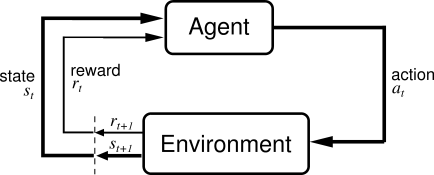
\includegraphics[width=0.6\textwidth]{assets/agent-env.png}
    \caption{MDP framework.}
    \label{fig:1}
\end{figure}

\subsection{Value function}

The Markov property states that the future state $s_{t+1}$ depends only on the current state $s_t$ and action $a_t$, 
and not on the previous states and actions.

\begin{equation}
    Pr(s_{t+1},r_t|s_t,a_t,s_{t-1},a_{t-1},...,s_0,a_0) = Pr(s_{t+1},r_t|s_t,a_t)
\end{equation}

Therefore, in an MDP, the expected return can be defined individually for each state $s \in S$, creating the concept of \textit{value function}. 

\begin{align}
    V_{\pi}(s) &= \mathbb{E}_{\pi}\left[r_t + \gamma r_{t+1} + \gamma^2 r_{t+2} + \dots | s_t = s\right] \\
    &= \sum_{a \in A}\pi(a|s) \sum_{s' \in S} \mathcal{P}(s'|s,a)\left[\mathcal{R}(s,a,s') + \gamma\mathbb{E}_{\pi}\left[u_{t+1}|s_{t+1}=s'\right]\right] \\
    &= \sum_{a \in A}\pi(a|s) \sum_{s' \in S} \mathcal{P}(s'|s,a)\left[\mathcal{R}(s,a,s') + \gamma V_{\pi}(s')\right]
\end{align}

This is referred to as the Bellman equation, and it defines a system of $m$ linear equations with $m$ variables ($m=|S|$) and a unique solution, given by the value function $V_{\pi}$ for policy $\pi$.
If all elements of the MDP are known, the value function can be computed by solving the system of equations. However, in most real-world scenarios, the transition probabilities and reward functions are unknown, and the agent must learn the value function through interaction with the environment.

\subsection{PPO}
Value-based RL methods are a class of RL algorithms that learn a value function, which is used to estimate the expected return of a state or state-action pair. The value function is usually represented as a neural network with parameters $\theta$, and it is updated using the Bellman equation. The value function can be used to derive a policy by selecting the action that maximizes the expected return.
The loss function is usually defined as squared error between the value function estimate and the target value $y_t$:
\begin{equation}
    \mathcal{L}(\theta) = \left(y_t - \mathcal{Q}(s_t,a_t;\theta)\right)
\end{equation}
where $y_t$ is the target value, defined as:
\begin{equation}
    y_t = \begin{cases}
        r_t + \gamma \max_{a'}\mathcal{Q}(s_{t+1},a_{t+1};\theta) & \text{if } s_{t+1} \text{ is not terminal} \\
        r_t & \text{if } s_{t+1} \text{ is terminal}
    \end{cases}
\end{equation}

Since the loss function contains the approximate value function twice, and we want to update the value estimate for the current state-action pair,
the solution is to stop any gradient flow backward through the target, to avoid computing gradients through the bootstrapped target value. In fact, 
the bootstrapped value estimate should only serve as a target value to optimize the main value estimate $\mathcal{Q}(s_t,a_t;\theta)$ toward.

To reduce the instability of training caused by the bootstrapped target value,
the target network is used, which is a different neural network with parameters $\phi$ that is used to compute bootstrapped target values.
Its parameters are periodically updated by copying the current parameters of the main value function network to the target network.
Another problem is the correlation of consecutive experiences. The update of value function parameters with most recent experiences may lead 
to the agent forgetting optimal policies learned in the past and in other experiences. This is due to the fact the changes in the policy will lead to 
changes in the data distribution encountered by the agent, which then lead to changes in the optimal policy. The usual solution is to randomize the experience samples used to train the agent,
that is why the replay buffer is used. In fact, a batch of experiences is sampled uniformly at random from the replay buffer, which will be used to 
update the value function parameters. This way, experiences can be reused multiple times (which leads to more efficient sampling) and gradients are more stable and with lower variance.

Policy gradient methods, instead, are a class of RL algorithms that learn a parameterized policy directly, without the need for a value function. The policy is usually represented as a neural network with parameters $\phi$, and it is updated using the policy gradient theorem. 
It provides a theoretically founded expression for the gradient of the performance of a parameterized policy with respect to the parameters of the policy.
\begin{equation}
    \nabla_{\phi}J(\phi) \propto \sum_{s\in \mathcal{S}}Pr(s|\pi)\sum_{a\in\mathcal{A}}Q^{\pi}(s,a)\nabla_{\phi}\pi(a|s;\phi)
\end{equation}

where $J$ represents a function measuring the quality of a policy $\pi$. It is similar to a loss function, but it is maximized and not minimized.
\begin{align}
    J(\phi) &= \mathbf{E}_{\pi}\left[\sum_{k}\gamma^k r_{t+k}\right] \\
            &= \sum_s Pr(s'|s,a)\sum_a\pi(a|s;\phi)\left[R_t+\gamma V_{\pi}(s_{t+1})\right]
\end{align}

Then, by writing the policy gradient as an expectation with respect to the probability of states occurring under the current policy and the probability of actions being selected by the policy:
\begin{equation}
    \nabla_{\phi}J(\phi) = \mathbf{E}_{s\sim Pr(\cdot|\pi),a\sim\pi(\cdot|s)}\left[Q^{\pi}(s,a)\nabla_{\phi}\log\pi(a|s;\phi)\right]
\end{equation}
This illustrates how the optimization of the parameterized policy is limited to on-policy only data.

The expectation in the policy gradient can be either approximated or obtained from samples. REINFORCE uses Monte Carlo estimation as a sampling method, which uses on-policy samples of episodic returns to approximate the expected returns of the policy.
It minimizes the following loss function:
\begin{equation}
    \mathcal{L}(\phi) = -\frac{1}{T}\sum_{t=0}^{T-1}\left(\sum_{\tau=t}^{T-1}\gamma^{\tau-t}r^{\tau}\right)\log \pi(a^t|s^t;\phi)
\end{equation}
Each episode, a full trajectory is collected by using current policy $\pi$, and then the return estimate is computed to estimate the policy gradient. 
However, Monte Carlo return estimates come with high variance and unstable training. Usually, the subtraction of a baseline (which keeps the bias but reduces the variance) is used as a solution.

Actor-critic algorithms train a parameterized policy (the actor) and a value function (the critic), alongside each other. The actor is optimized using gradient 
estimates derived from the policy gradient theorem, while the critic is used to compute bootstrapped return estimates. These estimates allow to estimate episodic 
returns just from the experience of a single step:
\begin{equation}
    \mathbf{E}_{s^t\sim Pr(\cdot|\pi)}\left[u(h^t)|s^t\right] = \mathbf{E}_{s^t\sim Pr(\cdot|\pi),a^t\sim\pi(\cdot|s^t),s^{t+1}\sim \mathcal{T}(\cdot|s^t,a^t)}\left[\mathcal{R}(s^t,a^t,s^{t+1}) + \gamma V(s^{t+1})|s^t\right]
\end{equation}
Moreover, bootstrapped return estimates exhibit lower variance compared to the Monte Carlo estimates of episodic returns, with the cost of introduced bias, since the value function might not approximate the true expected returns of states.
Essentially, a trade-off between bias and variance has to be made, and intermediate solutions are available just by estimating $N$-step returns, aggregating the received rewards of $N$ consecutive steps before computing a value estimate of the last state.

Advantages of the current policy can be computed to guide the policy gradients:
\begin{equation}
    Adv^{\pi}(s,a) = Q^{\pi}(s,a) - V^{\pi}(s)
\end{equation}
An advantage represents how much better or worse an action is compared to the average action in a given state. 
For a positive value, then, the probability of the policy $\pi$ choosing that action should be increased, while for a negative value it should be decreased. The advantage function can be estimated using the critic's value function as:
\begin{equation}
    Adv(s^t,a^t) = Q(s^t,a^t) - V(s^t) = \begin{cases} r^t + V(s^t) \quad \text{if }s^{t+1}\text{ is terminal} \\
    r^t + \gamma V(s^{t+1}) - V(s^t) \quad \text{otherwise}
    \end{cases}
\end{equation} 

Therefore, the actor loss to be minimized becomes:
\begin{equation}
    \mathcal{L}(\phi) = -Adv(s^t,a^t)\log\pi(a^t|s^t;\phi)
\end{equation}

And the critic loss is defined as:
\begin{equation}
    \mathcal{L}(\theta) = (y^t - V(s^t;\theta))^2
\end{equation}

Furthermore, entropy regularization can be added to the actor loss to discourage premature convergence to a suboptimal policy and incentivize exploration. 
It is a measure of the policy's uncertainty, and minimizing the negative entropy penalizes it for assigning a very high probability to any action.
\begin{equation}
    -\mathcal{H}(\pi(\cdot|s;\phi)) = \sum_{a\in\mathcal{A}}\pi(a|s;\phi)\log\pi(a|s;\phi)
\end{equation}

Since the individual gradient update steps could lead to large policy updates, the idea of Trust Regions was introduced in TRPO \cite{schulman2015trpo}, which 
essentially constrain the policy updates to a small area within the space of policy parameters in which the policy would not change significantly. 
PPO, instead, computes a computationally efficient surrogate objective to avoid large jumps in policy optimization steps. It makes use of importance sampling weights $\rho(s,a)$, which are defined
as the fraction of probabilities of selecting a given action $a$ in a state $s$ for two policies:
\begin{equation}
    \rho(s,a) = \frac{\pi(a|s;\phi)}{\pi_{\beta}(a|s)}
\end{equation}
This factor adjusts the data distribution to make the data generated by $\pi_{\beta}$ appear on-policy for $\pi$. Using these weights, PPO is able to update the policy multiple times using the same data and restrict the change of the policy by restricting the importance sampling weight.
In fact, the actor loss becomes:
\begin{equation}
    \mathcal{L}(\phi) = -\min \left(\rho(s^t,a^t)Adv(s^t,a^t), \text{clip}(\rho(s^t,a^t),1-\epsilon,1+\epsilon)Adv(s^t,a^t)\right)
\end{equation}

Algorithm~\ref{alg:ppo} summarize the whole procedure.

\begin{algorithm}[t]
\caption{PPO}
\label{alg:ppo}
\begin{algorithmic}[1]
\State Initialize actor network $\pi$ with random parameters $\phi$
\State Initialize critic network $V$ with random parameters $\theta$
\State Repeat for every episode:
\For{time step $t = 0,1,2,\dots$}
    \State Observe current state $s^t$
    \State Sample action $a^t \sim \pi(\cdot|s^t;\phi)$
    \State Apply action $a^t$; observe reward $r^t$ and next state $s^{t+1}$
    \State $\pi_{\beta}(a^t|s^t) \gets \pi(a^t|s^t;\phi)$ \Comment{store the old policy probability}
    \For{epoch $e=1,\dots,N_e$}
        \State $\rho(s^t,a^t) \gets \frac{\pi(a^t|s^t;\phi)}{\pi_{\beta}(a^t|s^t)}$
        \If{$s^{t+1}$ is terminal}
            \State Advantage $Adv(s^t,a^t)\gets r^t - V(s^t;\theta)$
            \State Critic target $y^t \gets r^t$
        \Else
            \State Advantage $Adv(s^t,a^t)\gets r^t + \gamma V(s^{t+1};\theta) - V(s^t;\theta)$
            \State Critic target $y^t \gets r^t + \gamma V(s^{t+1};\theta)$
        \EndIf
        \State Actor loss $\mathcal{L}(\phi)\gets -\min \left(\rho(s^t,a^t)Adv(s^t,a^t), \text{clip}(\rho(s^t,a^t),1-\epsilon,1+\epsilon)Adv(s^t,a^t)\right)$
        \State Critic loss $\mathcal{L}(\theta)\gets (y^t - V(s^t;\theta))^2$
        \State Update parameters $\phi$ by minimizing the actor loss $\mathcal{L}(\phi)$
        \State Update parameters $\theta$ by minimizing the critic loss $\mathcal{L}(\theta)$
    \EndFor
\EndFor
\end{algorithmic}
\end{algorithm}

\section{Multi-agent Reinforcement Learning}

When multiple agents are taken into consideration, the concept of Multi-agent Reinforcement Learning (MARL)
comes into play. In MARL, multiple agents interact with the same environment at the same time, and their 
actions can affect each other's rewards and state transitions. Moreover, each agent has its own long-term reward
to optimize, which now becomes a function of the policies of all other agents \cite{zhang2021multi}. 

\subsection{Markov Games}

Markov Games (MGs) are a generalization of MDPs to the multi-agent setting, and are defined by a tuple ($\mathcal{N}, \mathcal{S}, \left\{\mathcal{A}^i\right\}_{i\in\mathcal{N}}, \mathcal{P}, \left\{\mathcal{R}^i\right\}_{i\in\mathcal{N}}, \gamma$), where $\mathcal{N} = \left\{1,\dots,N\right\}$ denotes the set of agents, $\mathcal{S}$ denotes the state space observed by all agents, $\mathcal{A}^i$ denotes the action space of agent $i$.
Let $A:=A^1\times\dots\times A^N$ denote the joint action space, then $\mathcal{P}:\mathcal{S}\times \mathcal{A}\to\delta(\mathcal{S})$ denotes the transition probability function from any state $s\in\mathcal{S}$ to any state $s'\in\mathcal{S}$ for any joint action $a\in\mathcal{A}$; $R^i:\mathcal{S}\times\mathcal{A}\times\mathcal{S}\to\mathbb{R}$ is the reward function that determines the immediate reward received by agent $i$ for a transition from ($s,a$) to $s'$; $\gamma \in [0,1)$ is the discount factor.

At each time step $t$, each agent executes an action $a^i_t$ according to the system state $s_t$. The system transitions to a new state $s_{t+1}$ and gives each agent a reward $r^i_t$. Each agent wants to maximize its long-term reward, finding a policy $\pi^i$. As a consequence, the value-function $V^i : \mathcal{S}\to\mathbb{R}$ of agent $i$ becomes a function of the joint policy $\pi$ defined as $\pi(a|s) = \prod_{i\in\mathcal{N}}\pi^i(a^i|s)$.

\begin{equation}
    V^i_{\pi^i,\pi^{-i}} := \mathbb{E}\left[\sum_{t\geq 0}\gamma^t R^i(s_t,a_t,s_{t+1}) | a^i_t \sim \pi^i(\cdot | s_t), s_0 = s\right]
\end{equation}

Since each agent's value function depends on the policies of all other agents, the optimal policy for each agent is defined as a Nash equilibrium, where no agent can improve its long-term reward by unilaterally changing its policy.
A Nash equilibrium is a joint policy $\pi^* = (\pi^{1*},\dots,\pi^{N*})$ such that for all agents $i\in\mathcal{N}$ and for all states $s\in\mathcal{S}$, we have:

\begin{equation}
    V^i_{\pi^{i,*},\pi^{-i,*}}(s) \geq V^i_{\pi^i,\pi^{-i,*}}(s), \quad \forall \pi^i
\end{equation}

In other words, at a Nash equilibrium, each agent's policy is the best response to the policies of all other agents, and no agent can improve its long-term reward by changing its policy while the others keep theirs fixed.
It always exists for finite-space infinite-horizon discounted MGs, but may not be unique in general.

\subsection{Cooperative setting}

In some tasks, agent may need to cooperate to achieve a common goal, and in these cases they share a common reward function, i.e., $R^1 = R^2 = \dots = R^N = R$. 
With this model in mind, the value function and Q-function are identical to all agents, which thus enables the single-agent RL algorithms to be applied, if all agents are coordinated as one decision maker. 
Moreover, agents are allowed to have different reward functions, which may be kept private to each agent, while the goal for cooperation is to optimize the long-term reward corresponding to the average reward $\bar{R}(s,a,s') := N^{-1}\cdot\sum_{i\in\mathcal{N}}R^i(s,a,s')$ for any $(s,a,s')\in\mathcal{S}\times\mathcal{A}\times\mathcal{A}$. 

\subsection{Challenges of MARL}

MARL algorithms may be useful in many real-world applications, but they face several challenges that make them more difficult to design and analyze than single-agent RL algorithms.

\begin{itemize}
    \item \textbf{Non-stationarity}: since multiple agents learn concurrently, the environment faced by each agent is non-stationary, since the action taken by one agent affects the reward of other opponent agents, and the evolution of the state. As a result, each agent needs to learn to account for how other agents behave and adapt to the joint behavior accordingly. In fact, if each agent ignores this issue and optimizes its own policy assuming a stationary environment (\textit{independent learning}), the algorithms may fail to converge. 
    \item \textbf{Non-unique learning goals}: the learning goals in multi-agent settings may be unclear or conflicting, as each agent may have its own objectives and preferences, which may not align with those of other agents. This can lead to situations where agents are competing for resources or trying to achieve different goals, making it difficult to design algorithms that can effectively balance the needs of all agents.
    \item \textbf{Credit assignment problem}: in multi-agent settings, it can be difficult to determine which agent's actions contributed to the overall outcome, especially when the agents are working together towards a common goal. This can make it challenging to assign credit or blame for the success or failure of the team, and can lead to suboptimal learning outcomes.
    \item \textbf{Scalability}: to handle non-stationarity, each individual agent may need to account for the joint action space, whose dimension increases exponentially with the number of agents. This can make it difficult to scale MARL algorithms to large numbers of agents, as the computational and communication requirements may become prohibitive.
    \item \textbf{Partial observability}: in many real-world scenarios, agents may not have access to the full state of the environment, and may only be able to observe a limited subset of the state variables. This can make it difficult for agents to learn effective policies, as they may not have enough information to make informed decisions.
\end{itemize}
\chapter{Problem formulation}

A previous thesis \cite{insaghi2025thesis} already developed and analyzed 
a MARL algorithm suitable for this task. It used an environment made of
gaussians, which defined the reward function. However, the real world is 
more complex and made of currents. This thesis, thus, brings these contributions:
\begin{itemize}
    \item A new, more realistic environment, composed of currents, salinity and turbidity fields, created with Oceananigans;
    \item Another dimension to the problem, so that it goes from 2D to 3D;
    \item The use of a simulator, SwarmSwIM, to connect the environment with the agents and the MARL algorithm.
\end{itemize}

In the following sections, all those components are described in detail, 
including the parameters used to create the environment with the solver
and how agents are commanded via the simulator.

\section{SwarmSwIM Simulator}

SwarmSwIM \cite{swim_simulator} is a simulator developed to help researchers
and pratictioners to evaluate and enhance the control systems and decision-making
capabilities of underwater agents (AUVs). Completely Python-based, it provides
tools for current modeling, agent control and visual representation, balancing 
computational efficiency with sufficient environmental fidelity to facilitate large-scale
swarm simulations. The low-level control of the agents is approximated by the 
closed-loop control response of each agent, such as depth and heading keeping, in the 
resolution of the agent motion. 

Each member of the swarm is an \textit{agent} and is represented by a point
in the 3D space defined by the domain of the environment. The main cycle of it 
is made by simulation and agent ticks, where the former refers to the global update
while the latter to the local update of each agent. 

\section{Agent}

An agent is a point in the 3D space and its state is determined by four DoF: the 3D
position and the yaw angle. Roll and pitch are not considered, and yaw is fixed during 
an episode for simplicity. Agent control is achieved by three schemes:
\begin{enumerate}
    \item \textit{Depth}: Set to heave, such that the vertical velocity is taken as input;
    \begin{equation}
        z_{t+1} = (v_z + \epsilon) \Delta t + z_t \quad \text{with } \epsilon \sim \mathcal{N}(0, 1)
    \end{equation}
    \item \textit{Heading}: Set to yawrate but the yaw is always fixed;
    \begin{equation}
        \psi_{t+1} = (v_\psi + \epsilon) \Delta t + \psi_t 
    \end{equation}
    \item \textit{Planar}: Set to local velocity, such that current position is updated based on a velocity input command expressed in the body-frame reference system.
    \begin{equation}
        \begin{bmatrix}
            x_{t+1} \\
            y_{t+1} 
        \end{bmatrix} = 
        \begin{bmatrix}
            v_x + \epsilon \\
            v_y + \epsilon
        \end{bmatrix} \Delta t + 
        \begin{bmatrix}
            x_t \\
            y_t
        \end{bmatrix} 
    \end{equation}
\end{enumerate}

\section{Environment}

The environment is a 3D domain where the agents operate. To make it more realistic,
I used Oceananigans.jl \cite{Oceananigans-overview-paper-2025}, which is a 
fast, friendly and flexible software package for finite volume simulations of the 
nonhydrostatic and hydrostatic Boussinesq equations on CPUs and GPUs. An environment 
used in an episode is simply a snapshot of one of the different simulations
I ran with Oceananigans. The environment is composed of three fields:
\begin{itemize}
    \item \textit{Currents}
    \item \textit{Salinity}
    \item \textit{Turbidity}
\end{itemize}
The first one is computed by the solver. The second one is computed using
$N$ salinity sources, initialized randomly at "land" positions (i.e., south 
and west walls in this case) and with a random strength. The field is constructed 
by advecting the particles with the current field, corrected by a diffusion 
term. The third is simply an analytical function of depth:
\begin{equation}
    T(z) = \frac{1}{1 + e^{-(z - z_0)}} \quad \text{with } z_0 = 0.5
\end{equation}

The domain is a cube of $1000 \times 1000 \times 100$ meters, discretized
on a $128 \times 128 \times 64$ grid of cells, with topology (Periodic, Periodic, Bounded). The method chosen for the 
simulation is the nonhydrostatic one, which assumes that the vertical
acceleration is not negligible. This method is more accurate than the 
hydrostatic one, but necessitates more computational resources. 30 simulations
were carried out for training and 10 for testing, each one with a different random seed to ensure variability
in the environment. Each simulation created a single NetCDF file, with a snapshot
containing the fields every 12 minutes. The simulation was run for 18 hours,
with the first 12 used as warmup time and so not recorded. 

% Table with the parameters used for the simulation
\begin{table}[t]
\caption{Parameters used in the Oceananigans nonhydrostatic model\label{tab:1}}\vspace{0.25em} % adds some additional space between caption and \toprule, if desired.
\centering{%
\tagpdfsetup{table/header-rows={1}}
\begin{tabular*}{\textwidth}{@{\hspace*{1.5em}}@{\extracolsep{\fill}}ccc!{\hspace*{1.5em}}ccc@{\hspace*{5.0em}}}
\toprule
Parameter &
Value &
Description \\ \midrule
LX & 1000.0 & Domain (x) \\
LY & 1000.0 & Domain (y) \\
LZ & 100.0 & Domain (z) \\
NX & 128 & Grid points (x) \\
NY & 128 & Grid points (y) \\
NZ & 64 & Grid points (z) \\
$T_{surface}$ & 22.0 / 33.0 & Surface temperature (winter/summer) [°C]\\
$T_{bottom}$ & 20.0 / 22.0 & Bottom temperature (winter/summer) [°C]\\
$S_{baseline}$ & 40.0 / 42.0 & Baseline salinity (winter/summer) [PSU]\\
$V_{wind}$ & 5.0 / 8.0 & Wind speed (winter/summer) \\
$\rho_{air}$ & 1.225 & Air density [$kg/m^3$]\\
$c_{drag}$ & $1.3e^{-3}$ & Drag coefficient \\
$\rho_{water}$ & 1027.0 & Water density [$kg/m^3$]\\
Latitude & 24.5 & Abu Dhabi latitude (degrees N)\\
$\omega_{earth}$ & $7.292e^{-5}$ & Earth rotation rate [$rad/s$]\\
$f_{coriolis}$ & $2\omega_{earth}\sin(\text{Latitude})$ & Coriolis parameter [$rad/s$]\\
$\alpha_t$ & $1.67e^{-4}$ & Thermal expansion coefficient [$K^{-1}$]\\
$\beta_s$ & $0$ & Salinity contraction coefficient [$psu^{-1}$]\\
$\sigma_h$ & 300.0 & Salinity horizontal std [m]\\
$\sigma_v$ & 40.0 & Salinity vertical std [m]\\
Salinity excess & 10.0 & Excess over baseline [PSU]\\
Salinity decay time & 1.0 & Time to relax the field to a gaussian\\
Warmup time & 12.0 & Time to reach a steady state [h]\\
Simulation time & 6.0 & Total simulation time [h]\\
Output frequency & 12.0 & Frequency of output [min]\\
\bottomrule
\end{tabular*}
}%
\end{table}

\subsection{Currents}

Currents are composed by three components: the horizontal velocities ($u,v$),
and the vertical one ($w$). They are prognostic variables integrated 
forward in time by the nonhydrostatic Oceananigans model, which solves the rotating, 
Boussinesq, nonhydrostatic Navier–Stokes equations with an LES subgrid closure. 
The developed script only sets up the forcing, the boundary conditions, the rotation, 
the stratification, and the time-stepping; the flow itself emerges from the solve.
The model integrates the following equation:

\begin{equation}
\frac{\partial \mathbf{\vec{u}}}{\partial t} + \underbrace{(\mathbf{\vec{u}}\cdot\nabla)\mathbf{\vec{u}}}_{\text{advection}} + \underbrace{f \hat{z}\times\mathbf{\vec{u}}}_{\text{coriolis}} = -\underbrace{\nabla p}_{\text{pressure}} + \underbrace{b \hat{z}}_{\text{buoyancy}} + \underbrace{\nabla\cdot\boldsymbol{\tau}_{\rm sgs}}_{\text{subgrid stress}} + \underbrace{\mathbf{F}}_{\text{body force}}
\end{equation}

\begin{equation*}
    \text{with } \nabla\cdot\mathbf{\vec{u}} = 0
\end{equation*}

The fourth term $(-\nabla p)$ is the pressure gradient force. It is a global 
operator (i.e., modifies the entire domain) and essentially is a vector
pointing in the direction of steepest increase in pressure. Because the model 
is Boussinesq, $p$ here is the kinemaic pressure, already divided by $\rho_0 = 1027.0$. 
Moreover, it has no equation of state, it is a Lagrange multiplier that enforces incompressibility, 
and since there is the constraint $\nabla\cdot\mathbf{\vec{u}} = 0$, it is whatever force field 
required to make that true. Mechanically, Oceananigans does thig with a projection
method each timestep:
\begin{itemize}
    \item advances velocity ignoring pressure
    \item solves a Poisson equation for pressure
    \begin{equation}
        \nabla^2 p = \nabla\cdot \mathbf{\vec{u}}^* / \Delta t
    \end{equation}
    \item corrects the velocity with the pressure gradient
    \begin{equation}
        \vec{u} = \vec{u}^* - \Delta t \cdot \nabla p
    \end{equation}
\end{itemize}
The second step is an elliptic solve that uses an FFT along the periodi axis and transforms along the bounded axes.

The fifth term ($b\hat{z}$) is the buoyancy force, TODO.

The sixth term ($\nabla\cdot\boldsymbol{\tau}_{\rm sgs}$) is the subgrid stress, which is a closure for the unresolved scales of motion. 
Essentially, LES applies a spatial filter (the grid) to the Navier-Stokes equations, splitting the velocity into a resolved and an unresolved part.
Physically, $\tau_{\rm sgs}$ is the momentum flux carried by eddies smaller than a grid cell, since in the current model the grid cells cannot see them. 

The last term ($\mathbf{F}$) embodies every forcing that is not in the standard list of fixed physics solved by Oceananigans.
It is a body force, applied throughout the volume at every grid cell. 

Wind speed enters whrough the bulk drag law:
\begin{equation}
\tau = \rho_{\rm air},C_d,U_{10}^2 \quad\Longrightarrow\quad \tau_{\rm kin} = \frac{\rho_{\rm air} C_d U_{10}^2}{\rho_{\rm water}}
\end{equation}

And that is applied as a flux boundary condition at the surface. Momentum enters through the surface and
is transferred downward by turbulence. 
Surface stress plus rotation gives the classical Ekman spiral: the current at the surface
is deflected to the right of the wind (northern hemisphere) and rotates further right with depth while decaying. 

Only temperature is buoyancy-active: salinity exerts zero feedback on momentum, it is advected and LES-mixed by the currents but never drives them.
This is a simplification with respect to the real world, given the small amount of computational resources available.



\subsection{Salinity Field}
\chapter{Proposed Method}

The task at hand can be described as target area search and navigation in an unknown environment. 
This task is currently being addressed in the literature, even though there is not a specific
area of research that focuses on it. In fact, different authors have considered using MARL solutions
to target localization, path planning and source seeking problems. 

TODO: mention other works and explain them.

The novelty of this work, in fact,
is the use of MARL algorithms to search a specific target area, specified by some parameters that in 
this case are the turbidity and the salinity. To do so, IPPO \cite{dewitt2020ippo} and MAPPO \cite{yu2022mappo} have been 
chosen as first approaches to solve the problem, given their popularity and effectiveness in multi-agent scenarios. The following sections will describe 
them in detail. 

\section{Agent State}

\section{Reward Function}

\section{IPPO}

Independent Proximal Policy Optimization (IPPO) is the multi-agent version of the popular Proximal Policy Optimization (PPO) algorithm \cite{schulman2017ppo}, 
an on-policy RL algorithm that uses a clipped surrogate objective to update the policy. In IPPO, each agent is used to learn a common policy, so the agents share
its parameters. It is like having $N$ independent agents each with the same PPO-trained policy on a single-agent scenario,
but the use of shared parameters helps having a more efficient sampling since in an episode multiple gradients are computed and used from different parts of the environment.

In IPPO, a variant of the advantage function is used, where each agent learns a local observation based critic $V_{\phi}(z^a_t)$ parameterised by $\phi$ using \textit{Generalized Advantage Estimation (GAE)}. For each agent
$a$, the relative advantage function is defined as:
\begin{equation}
    A^a_t = \sum_{l=0}^{h}(\gamma\lambda)^l\delta^a_{t+l}
\end{equation}
where $\delta^a_t = r^a_t + \gamma V_{\phi}(z^a_{t+1}) - V_{\phi}(z^a_t)$ is the temporal difference error, $\gamma$ is the discount factor and $\lambda$ is a hyperparameter that controls the bias-variance trade-off of the advantage estimates.
The final policy loss for each agent is defined as:
\begin{equation}
    \mathcal{L}^a(\theta) = \mathbf{E}_{z^a_t,u^a_t}\left[\min\left(\frac{\pi_{\theta}(u^a_t|z^a_t)}{\pi_{\theta_{old}}(u^a_t|z^a_t)}A^a_t,\text{ clip }\left(\frac{\pi_{\theta}(u^a_t|z^a_t)}{\pi_{\theta_{old}}(u^a_t|z^a_t)},1-\epsilon,1+\epsilon\right)A^a_t\right)\right]
\end{equation}

The full procedure is summarized in Algorithm~\ref{alg:ippo}. Since the parameters are shared, the transitions collected
by the $n$ agents are flattened into a single batch and treated as independent samples of the same policy: one iteration
alternates a rollout phase, in which the behaviour policy $\pi_{\theta_{old}}$ is kept fixed, and an optimization phase,
in which the same batch is reused for $K$ epochs over $M$ minibatches. A binary mask $m^a_t$ excludes from the loss the
steps of agents that have already terminated their episode, so that frozen agents do not contribute spurious gradients.

\begin{algorithm}[t]
\caption{IPPO}
\label{alg:ippo}
\begin{algorithmic}[1]
\Require actor parameters $\theta$, critic parameters $\phi$; $n$ agents; $E$ parallel environments; rollout length $T$;
         epochs $K$; minibatches $M$; clipping parameter $\epsilon$; discount $\gamma$; GAE parameter $\lambda$;
         coefficients $\lambda_{critic},\lambda_{entropy}$; KL threshold $\kappa$
\Ensure trained policy $\pi_\theta$
\State Initialize $\theta,\phi$ using Orthogonal initialization
\While{$step\leq step_{max}$}
    \State $\theta_{old} \gets \theta$, \quad $\phi_{old} \gets \phi$ \Comment{freeze the behaviour policy}
    \For{$t = 0,\dots,T-1$} \Comment{rollout phase, no gradient tracking}
        \ForAll{agents $a$ in each environment}
            \State sample $u^a_t \sim \pi_{\theta_{old}}(\cdot\,|\,z^a_t)$ and store $\log\pi_{\theta_{old}}(u^a_t|z^a_t)$ and $V_{\phi_{old}}(z^a_t)$
        \EndFor
        \State step the environments and observe $r^a_t$, $z^a_{t+1}$ and the termination flags $d^a_{t+1}$
        \State store the transition together with the mask $m^a_t = 1 - d^a_t$
    \EndFor
    \For{$t = T-1,\dots,0$} \Comment{GAE, bootstrapped from $V_{\phi_{old}}(z^a_T)$}
        \State $\delta^a_t \gets r^a_t + \gamma\,(1-d^a_{t+1})\,V_{\phi_{old}}(z^a_{t+1}) - V_{\phi_{old}}(z^a_t)$
        \State $A^a_t \gets \delta^a_t + \gamma\lambda\,(1-d^a_{t+1})\,A^a_{t+1}$, \quad $\hat{V}^a_t \gets A^a_t + V_{\phi_{old}}(z^a_t)$
    \EndFor
    \State flatten the $T\cdot E\cdot n$ agent-steps into a single batch $\mathcal{B}$
    \For{epoch $k = 1,\dots,K$}
        \ForAll{minibatches $b \subset \mathcal{B}$ of size $|\mathcal{B}|/M$}
            \State normalize the advantages $A^a_t$ over $b$ to zero mean and unit variance
            \State evaluate $\mathcal{L}(\theta,\phi)$ on $b$, averaging every term with the masks $m^a_t$
            \State update $\theta,\phi$ by gradient ascent on $\mathcal{L}(\theta,\phi)$ (Adam, clipped gradient norm)
        \EndFor
        \If{$\widehat{\mathrm{KL}}\big(\pi_{\theta_{old}}\Vert\pi_{\theta}\big) > \kappa$}
            \State \textbf{break} \Comment{early stopping on excessive policy change}
        \EndIf
    \EndFor
\EndWhile
\end{algorithmic}
\end{algorithm}

\begin{table}[t]
\caption{Default env parameters\label{tab:env_params}}\vspace{0.25em} % adds some additional space between caption and \toprule, if desired.
\centering{%
\tagpdfsetup{table/header-rows={1}}
\begin{tabular*}{0.6\textwidth}{@{\hspace*{3.0em}}@{\extracolsep{\fill}}ccc!{\hspace*{3.0em}}ccc@{\hspace*{2.0em}}}
\toprule
Parameter &
Value \\ \midrule
$\epsilon_{S}$ & 0.15 \\
$\epsilon_{\Tau}$ & 0.05 \\
$\sigma_{S}$ & 1.5 \\
$\sigma_{\Tau}$ & 0.3 \\
n\_agents & 2 \\
k & 12 \\
v\_agent & 1.0 \\
max\_steps & 1800 \\
$\delta t$ & 0.1 \\
frame\_skip & 10 \\
success\_bonus & 20.0 \\
\bottomrule
\end{tabular*}
}%
\end{table}

\begin{table}[t]
\caption{IPPO parameters\label{tab:ippo_params}}\vspace{0.25em} % adds some additional space between caption and \toprule, if desired.
\centering{%
\tagpdfsetup{table/header-rows={1}}
\begin{tabular*}{0.6\textwidth}{@{\hspace*{3.0em}}@{\extracolsep{\fill}}ccc!{\hspace*{3.0em}}ccc@{\hspace*{2.0em}}}
\toprule
Parameter &
Value \\ \midrule
total\_timesteps & 10M \\
learning\_rate & 0.0003 \\
num\_envs & 12 \\
num\_steps & 512 \\
anneal\_lr & False \\
$\gamma$ & 0.9995 \\
$\lambda_{GAE}$ & 0.95 \\
$num\_minibatches$ & 24 \\
update\_epochs & 10 \\
norm\_adv & True \\
clip\_coeff & 0.25 \\
clip\_vloss & False \\
entropy\_coef & 0.01 \\
anneal\_entropy & True \\
ent\_anneal\_frac & 0.5 \\
ent\_coef\_final & 0.0 \\
vf\_coef & 0.5 \\
max\_grad\_norm & 0.5 \\
target\_kl & 0.02 \\
\bottomrule
\end{tabular*}
}%
\end{table}

\section{MAPPO}

\begin{algorithm}[t]
\caption{MAPPO}
\label{alg:mappo}
\begin{algorithmic}[1]
\Require actor parameters $\theta$, critic parameters $\phi$; $n$ agents; $E$ parallel environments; rollout length $T$;
         epochs $K$; minibatches $M$; clipping parameter $\epsilon$; discount $\gamma$; GAE parameter $\lambda$;
         coefficients $\lambda_{critic},\lambda_{entropy}$; KL threshold $\kappa$
\Ensure trained policy $\pi_\theta$
\State Initialize $\theta,\phi$ using Orthogonal initialization
\State Set learning rate $\alpha$ and decay schedule
\While{$step\leq step_{max}$}
    \State set data buffer $D = {}$
    \For{$i = 1,\dots,\text{batch size}$} 
        \State $\tau = []$
        \State initialize $h^{(1)}_{0,\pi},\dots,h^{(n)}_{0,\pi}$ actor states
        \State initialize $h^{(1)}_{0,V},\dots,h^{(n)}_{0,V}$ critic states
        \For{$t = 1,\dots,T$}
            \ForAll{agents $a$}
                \State $p^{(a)}_t,h^{(a)}_{t,\pi} = \pi(o^{(a)}_t,h^{(a)}_{t+1,\pi};\theta)$
                \State $u^{(a)}_t \sim p^{(a)}_t$
                \State $v^{(a)}_t,h^{(a)}_{t,V} = V(o^{(a)}_t,h^{(a)}_{t+1,V};\phi)$
            \EndFor
            \State Execute actions $u_t$, observe $r_t,s_{t+1},o_{t+1}$
            \State $\tau += \left[s_t,o_t,h_{t,V},u_t,r_t,s_{t+1},o_{t+1}\right]$
        \EndFor
    \EndFor
    \For{$t = T-1,\dots,0$} \Comment{GAE, bootstrapped from $V$}
        \State $\delta^a_t \gets r^a_t + \gamma\,(1-d^a_{t+1})\,V_{\phi_{old}}(z^a_{t+1}) - V_{\phi_{old}}(z^a_t)$
        \State $A^a_t \gets \delta^a_t + \gamma\lambda\,(1-d^a_{t+1})\,A^a_{t+1}$, \quad $\hat{V}^a_t \gets A^a_t + V_{\phi_{old}}(z^a_t)$
    \EndFor
    \State flatten the $T\cdot E\cdot n$ agent-steps into a single batch $\mathcal{B}$
    \For{epoch $k = 1,\dots,K$}
        \ForAll{minibatches $b \subset \mathcal{B}$ of size $|\mathcal{B}|/M$}
            \State normalize the advantages $A^a_t$ over $b$ to zero mean and unit variance
            \State evaluate $\mathcal{L}(\theta,\phi)$ on $b$, averaging every term with the masks $m^a_t$
            \State update $\theta,\phi$ by gradient ascent on $\mathcal{L}(\theta,\phi)$ (Adam, clipped gradient norm)
        \EndFor
        \If{$\widehat{\mathrm{KL}}\big(\pi_{\theta_{old}}\Vert\pi_{\theta}\big) > \kappa$}
            \State \textbf{break} \Comment{early stopping on excessive policy change}
        \EndIf
    \EndFor
\EndWhile
\end{algorithmic}
\end{algorithm}
\chapter{Experiments}

This chapter includes all the experiments that were 
performed to test the obtained policies in different 
contexts.
\chapter{Conclusions and Future Work}

This work presented a comprehensive study on the application of Multi-Agent Reinforcement Learning (MARL)
approaches to the problem of underwater search and navigation in an unknown, realistic and complex environment.
The study focused on the application of multi-agent PPO variants, especially IPPO and MAPPO, with the addition of a 
communication mechanism to enhance the agents' performance in a partially observable environment. The results demonstrated
the effectiveness of the proposed approaches in making the agents find the target area in the shortest amount of time. 
Different approaches lead to different results, even though independent agents are optimal choice if there is not prior 
information regarding the environment. In fact, the use of communication has been proved to help in difficult scenarios and
in situations where agents are spread and thus find helpful having knowledge about other points in the environment,
whether if they start close it does not help much. The centralized critic was not generally found helpful in this task,
even though in some cases it helped achieving a better performance, especially with a lower number of agents and with a 
smaller target area. 
In this problem, since the target is defined as an area and usually it is quite large, training a policy with more than 2 agents
was difficult and not optimal. Increasing to 4 agents, in fact, showed that independence leads to better performances overall, which is 
different from what one might expect. The effect of lucky spawning near the target zone, more probable in this case,
has led to an optimal policy which favors the removal of communication, probably because using a larger state does not bring 
any advance with respect to the independent case, which is comprehensible.
Efficiency is measured as the time to reach success, and in this task independent agents reached the worst performance overall, 
while MAPPO is the most efficient policy with 2 agents. This is explained by the fact that agents trained with a centralized policy
are able to divide the work more efficiently than independent agents, which only care about success and reaching target. Coordinated agents,
instead, trade some success for more efficiency, and that is proved by the time they take to reach the target zone. 
Finally, the way agents are initialized has been found to matter a lot,
and the verdict is to use a uniform initialization to encode a natural spread in the environment. This could be informative for 
real deployment consideration, since it is not said that the cost of releasing the AUVs spread is lower than the what the difference in 
success rate brings, and that should be defined beforehand.

This problem is inherently difficult, since the target area depends on how the environment is made up and which variables
are considered. In fact, in this case only two parameters are considered for the target, but there could be more. Adding more 
constraints naturally complicates the learning problem, and there could be no optimal policy to navigate the environment in that case,
since the more the variables that need to be taken into consideration, the more difficult would be for the agent to navigate using gradients
and the higher will be the dimension of the state space. However, this should be the very next starting point for further analyze the effect 
of scaling the number of agents, since the dimension of the target area resulted to be the main problem that limited the 
training of an optimal policy with more than 2 agents. Moreover, 
other forms of communication and cooperation could be exploited and tested, for example with swarm capabilities that in this case were unhelpful due to the 
small environment and number of agents considered. If a larger number of agents are used, which complicates even further the learning 
problem, the consideration of techniques like PSO could help the agents avoid local optima generated from the more complex environment,
since those techniques are more effective with large swarms. 

To conclude, learning optimal policies in this task is definitely possible, even though the complexity of the real environment 
may be much higher than a simulated one like the one developed in this work. In fact, obstacles may be present and unexpected hazards
are possible and should be taken into account. This work proved that MARL is a promising approach to solve problems in the underwater domain,
like coral reef restoration and monitoring, which are vital for the health of the marine ecosystem. Further optimizations and improvements are needed 
to make the proposed approaches more robust and effective in real-world scenarios, but the results obtained in this work provide a solid foundation for future research in this area.


%%% Appendices of thesis  %%%%%%%%%%%%%%%%%%%%%%%%%%%%%%%%%%%%%%%%%%%%%%%%%%%%%%%%%%%%%%%%%%%%%%%%

\appendix
%\include{appendixa}% listings example (not compatible with tagged pdf, as of June 2026)
%\include{appendixb}% longtable example


%%% Bibliography (biblatex)  %%%%%%%%%%%%%%%%%%%%%%%%%%%%%%%%%%%%%%%%%%%%%%%%%%%%%%%%%%%%%%%%%%%%%%

\defbibheading{bibintoc}{\chapter*{#1}\addcontentsline{toc}{backmatter}{\refname}} 
% this sets the title of contents name for bibliography to \refname (= References)
% change "backmatter" to "chapter" if you prefer a bold face entry in the table of contents

\printbibliography[title={\refname},heading=bibintoc]

% biblatex also supports chapter-by-chapter bibliography, https://tex.stackexchange.com/a/296502/119566
% see the biblatex manual, section 3.14.3


\end{document} 
 